% !TeX program = xelatex 
%  LaTeX support: latex@mdpi.com 
%  For support, please attach all files needed for compiling as well as the log file, and specify your operating system, LaTeX version, and LaTeX editor.

%=================================================================
\documentclass[mathematics,article,submit,moreauthors]{Definitions/mdpi} 

%--------------------
% Class Options:
%--------------------
%----------
% journal
%----------
% Choose between the following MDPI journals:
% acoustics, actuators, addictions, admsci, adolescents, aerobiology, aerospace, agriculture, agriengineering, agrochemicals, agronomy, ai, air, algorithms, allergies, alloys, analytica, analytics, anatomia, animals, antibiotics, antibodies, antioxidants, applbiosci, appliedchem, appliedmath, applmech, applmicrobiol, applnano, applsci, aquacj, architecture, arm, arthropoda, arts, asc, asi, astronomy, atmosphere, atoms, audiolres, automation, axioms, bacteria, batteries, bdcc, behavsci, beverages, biochem, bioengineering, biologics, biology, biomass, biomechanics, biomed, biomedicines, biomedinformatics, biomimetics, biomolecules, biophysica, biosensors, biotech, birds, bloods, blsf, brainsci, breath, buildings, businesses, cancers, carbon, cardiogenetics, catalysts, cells, ceramics, challenges, chemengineering, chemistry, chemosensors, chemproc, children, chips, cimb, civileng, cleantechnol, climate, clinpract, clockssleep, cmd, coasts, coatings, colloids, colorants, commodities, compounds, computation, computers, condensedmatter, conservation, constrmater, cosmetics, covid, crops, cryptography, crystals, csmf, ctn, curroncol, cyber, dairy, data, ddc, dentistry, dermato, dermatopathology, designs, devices, diabetology, diagnostics, dietetics, digital, disabilities, diseases, diversity, dna, drones, dynamics, earth, ebj, ecologies, econometrics, economies, education, ejihpe, electricity, electrochem, electronicmat, electronics, encyclopedia, endocrines, energies, eng, engproc, entomology, entropy, environments, environsciproc, epidemiologia, epigenomes, est, fermentation, fibers, fintech, fire, fishes, fluids, foods, forecasting, forensicsci, forests, foundations, fractalfract, fuels, future, futureinternet, futurepharmacol, futurephys, futuretransp, galaxies, games, gases, gastroent, gastrointestdisord, gels, genealogy, genes, geographies, geohazards, geomatics, geosciences, geotechnics, geriatrics, grasses, gucdd, hazardousmatters, healthcare, hearts, hemato, hematolrep, heritage, higheredu, highthroughput, histories, horticulturae, hospitals, humanities, humans, hydrobiology, hydrogen, hydrology, hygiene, idr, ijerph, ijfs, ijgi, ijms, ijns, ijpb, ijtm, ijtpp, ime, immuno, informatics, information, infrastructures, inorganics, insects, instruments, inventions, iot, j, jal, jcdd, jcm, jcp, jcs, jcto, jdb, jeta, jfb, jfmk, jimaging, jintelligence, jlpea, jmmp, jmp, jmse, jne, jnt, jof, joitmc, jor, journalmedia, jox, jpm, jrfm, jsan, jtaer, jvd, jzbg, kidneydial, kinasesphosphatases, knowledge, land, languages, laws, life, liquids, literature, livers, logics, logistics, lubricants, lymphatics, machines, macromol, magnetism, magnetochemistry, make, marinedrugs, materials, materproc, mathematics, mca, measurements, medicina, medicines, medsci, membranes, merits, metabolites, metals, meteorology, methane, metrology, micro, microarrays, microbiolres, micromachines, microorganisms, microplastics, minerals, mining, modelling, molbank, molecules, mps, msf, mti, muscles, nanoenergyadv, nanomanufacturing,\gdef\@continuouspages{yes}} nanomaterials, ncrna, ndt, network, neuroglia, neurolint, neurosci, nitrogen, notspecified, %%nri, nursrep, nutraceuticals, nutrients, obesities, oceans, ohbm, onco, %oncopathology, optics, oral, organics, organoids, osteology, oxygen, parasites, parasitologia, particles, pathogens, pathophysiology, pediatrrep, pharmaceuticals, pharmaceutics, pharmacoepidemiology,\gdef\@ISSN{2813-0618}\gdef\@continuous pharmacy, philosophies, photochem, photonics, phycology, physchem, physics, physiologia, plants, plasma, platforms, pollutants, polymers, polysaccharides, poultry, powders, preprints, proceedings, processes, prosthesis, proteomes, psf, psych, psychiatryint, psychoactives, publications, quantumrep, quaternary, qubs, radiation, reactions, receptors, recycling, regeneration, religions, remotesensing, reports, reprodmed, resources, rheumato, risks, robotics, ruminants, safety, sci, scipharm, sclerosis, seeds, sensors, separations, sexes, signals, sinusitis, skins, smartcities, sna, societies, socsci, software, soilsystems, solar, solids, spectroscj, sports, standards, stats, std, stresses, surfaces, surgeries, suschem, sustainability, symmetry, synbio, systems, targets, taxonomy, technologies, telecom, test, textiles, thalassrep, thermo, tomography, tourismhosp, toxics, toxins, transplantology, transportation, traumacare, traumas, tropicalmed, universe, urbansci, uro, vaccines, vehicles, venereology, vetsci, vibration, virtualworlds, viruses, vision, waste, water, wem, wevj, wind, women, world, youth, zoonoticdis 
% For posting an early version of this manuscript as a preprint, you may use "preprints" as the journal. Changing "submit" to "accept" before posting will remove line numbers.

%---------
% article
%---------
% The default type of manuscript is "article", but can be replaced by: 
% abstract, addendum, article, book, bookreview, briefreport, casereport, comment, commentary, communication, conferenceproceedings, correction, conferencereport, entry, expressionofconcern, extendedabstract, datadescriptor, editorial, essay, erratum, hypothesis, interestingimage, obituary, opinion, projectreport, reply, retraction, review, perspective, protocol, shortnote, studyprotocol, systematicreview, supfile, technicalnote, viewpoint, guidelines, registeredreport, tutorial
% supfile = supplementary materials

%----------
% submit
%----------
% The class option "submit" will be changed to "accept" by the Editorial Office when the paper is accepted. This will only make changes to the frontpage (e.g., the logo of the journal will get visible), the headings, and the copyright information. Also, line numbering will be removed. Journal info and pagination for accepted papers will also be assigned by the Editorial Office.

%------------------
% moreauthors
%------------------
% If there is only one author the class option oneauthor should be used. Otherwise use the class option moreauthors.

%---------
% pdftex
%---------
% The option pdftex is for use with pdfLaTeX. Remove "pdftex" for (1) compiling with LaTeX & dvi2pdf (if eps figures are used) or for (2) compiling with XeLaTeX.

%=================================================================
% MDPI internal commands - do not modify
\firstpage{1} 
\makeatletter 
\setcounter{page}{\@firstpage} 
\makeatother
\pubvolume{1}
\issuenum{1}
\articlenumber{0}
\pubyear{2023}
\copyrightyear{2023}
%\externaleditor{Academic Editor: Firstname Lastname}
\datereceived{ } 
\daterevised{ } % Comment out if no revised date
\dateaccepted{ } 
\datepublished{ } 
%\datecorrected{} % For corrected papers: "Corrected: XXX" date in the original paper.
%\dateretracted{} % For corrected papers: "Retracted: XXX" date in the original paper.
\hreflink{https://doi.org/} % If needed use \linebreak
%\doinum{}
%\pdfoutput=1 % Uncommented for upload to arXiv.org

%=================================================================
% Add packages and commands here. The following packages are loaded in our class file: fontenc, inputenc, calc, indentfirst, fancyhdr, graphicx, epstopdf, lastpage, ifthen, float, amsmath, amssymb, lineno, setspace, enumitem, mathpazo, booktabs, titlesec, etoolbox, tabto, xcolor, colortbl, soul, multirow, microtype, tikz, totcount, changepage, attrib, upgreek, array, tabularx, pbox, ragged2e, tocloft, marginnote, marginfix, enotez, amsthm, natbib, hyperref, cleveref, scrextend, url, geometry, newfloat, caption, draftwatermark, seqsplit
% cleveref: load \crefname definitions after \begin{document}

%=================================================================
% Please use the following mathematics environments: Theorem, Lemma, Corollary, Proposition, Characterization, Property, Problem, Example, ExamplesandDefinitions, Hypothesis, Remark, Definition, Notation, Assumption
%% For proofs, please use the proof environment (the amsthm package is loaded by the MDPI class).

%=================================================================
% Full title of the paper (Capitalized)
%\Title{Expansive Information Injection with Large Language Models for Multi-Span Question Answering }
\Title{Empowering Multi-Span Question Answering with Expansive Information Injection using Large Language Models}

% MDPI internal command: Title for citation in the left column
\TitleCitation{Title}

% Author Orchid ID: enter ID or remove command
\newcommand{\orcidauthorA}{0000-0002-2206-1926} % Add \orcidA{} behind the author's name
%\newcommand{\orcidauthorB}{0000-0000-0000-000X} % Add \orcidB{} behind the author's name


% Authors, for the paper (add full first names)
\Author{Zhiyi Luo $^{1}$\orcidA{}, Yingying Zhang$^{1}$ and Shuyun Luo $^{1,}$*}

%\longauthorlist{yes}

% MDPI internal command: Authors, for metadata in PDF
\AuthorNames{Zhiyi Luo, Yingying Zhang and Shuyun Luo}

% MDPI internal command: Authors, for citation in the left column
\AuthorCitation{Luo, Z.; Zhang, Y.; Luo, S.}
% If this is a Chicago style journal: Lastname, Firstname, Firstname Lastname, and Firstname Lastname.

% Affiliations / Addresses (Add [1] after \address if there is only one affiliation.)
\address{%
$^{1}$ \quad School of Computer Science and Technology and the Key Laboratory of Intelligent Textile and Flexible Interconnection of Zhejiang Province, Zhejiang Sci-Tech University, Hangzhou, China; luozhiyi@zstu.edu.cn
%$^{2}$ \quad Affiliation 2; e-mail@e-mail.com
}

% Contact information of the corresponding author
\corres{Correspondence: shuyunluo@zstu.edu.cn;}

% Current address and/or shared authorship
%\firstnote{Current address: Affiliation 3.} 
%\secondnote{These authors contributed equally to this work.}
% The commands \thirdnote{} till \eighthnote{} are available for further notes

%\simplesumm{} % Simple summary

%\conference{} % An extended version of a conference paper

% Abstract (Do not insert blank lines, i.e. \\) 
\abstract{Retrieval-based question answering in the automotive domain requires a model to comprehend and articulate relevant domain knowledge, accurately understand user intent, and effectively match the required information. Typically, these systems employ a encoder-retriever architecture. However, existing encoders, which rely on pretrained language models, suffer from limited specialization, insufficient awareness of domain knowledge, and biases in user intent understanding. To overcome these limitations, this paper constructs a Chinese corpus specifically tailored for the automotive domain, comprising question-answer pairs, document collections, and multitask annotated data. Subsequently, a pretraining-multitask fine-tuning framework based on masked language models is introduced to integrate domain knowledge as well as enhance semantic representations, thereby yielding benefits for downstream applications. To evaluate system performance, an evaluation dataset is created using ChatGPT, and a novel retrieval task evaluation metric called Mean Linear Window Rank (MLWR) is proposed. Experimental results demonstrate that the proposed system (based on $\text{BERT}_{base}$), achieves accuracies of 77.5\% and 84.75\% for Hit@1 and Hit@3 respectively, in the automotive domain retrieval-based question answering task. Additionally, the MLWR reaches 87.71\%. Compared to a system utilizing a general encoder, the proposed multitask fine-tuning strategy shows improvements of 12.5\%, 12.5\%, and 28.16\% for Hit@1, Hit@3, and MLWR, respectively. Furthermore, when compared to the best single-task fine-tuning strategy, the enhancements amount to 0.5\%, 1.25\%, and 0.95\% for Hit@1, Hit@3, and MLWR, respectively.}

% Keywords
\keyword{deep learning; pretrained language model; retrieval-based question answering; multitask learning; fine-tuning} 

% The fields PACS, MSC, and JEL may be left empty or commented out if not applicable
%\PACS{J0101}
%\MSC{}
%\JEL{}

%%%%%%%%%%%%%%%%%%%%%%%%%%%%%%%%%%%%%%%%%%
% Only for the journal Diversity
%\LSID{\url{http://}}

%%%%%%%%%%%%%%%%%%%%%%%%%%%%%%%%%%%%%%%%%%
% Only for the journal Applied Sciences
%\featuredapplication{Authors are encouraged to provide a concise description of the specific application or a potential application of the work. This section is not mandatory.}
%%%%%%%%%%%%%%%%%%%%%%%%%%%%%%%%%%%%%%%%%%

%%%%%%%%%%%%%%%%%%%%%%%%%%%%%%%%%%%%%%%%%%
% Only for the journal Data
%\dataset{DOI number or link to the deposited data set if the data set is published separately. If the data set shall be published as a supplement to this paper, this field will be filled by the journal editors. In this case, please submit the data set as a supplement.}
%\datasetlicense{License under which the data set is made available (CC0, CC-BY, CC-BY-SA, CC-BY-NC, etc.)}

%%%%%%%%%%%%%%%%%%%%%%%%%%%%%%%%%%%%%%%%%%
% Only for the journal Toxins
%\keycontribution{The breakthroughs or highlights of the manuscript. Authors can write one or two sentences to describe the most important part of the paper.}

%%%%%%%%%%%%%%%%%%%%%%%%%%%%%%%%%%%%%%%%%%
% Only for the journal Encyclopedia
%\encyclopediadef{For entry manuscripts only: please provide a brief overview of the entry title instead of an abstract.}

%%%%%%%%%%%%%%%%%%%%%%%%%%%%%%%%%%%%%%%%%%
% Only for the journal Advances in Respiratory Medicine
%\addhighlights{yes}
%\renewcommand{\addhighlights}{%

%\noindent This is an obligatory section in “Advances in Respiratory Medicine”, whose goal is to increase the discoverability and readability of the article via search engines and other scholars. Highlights should not be a copy of the abstract, but a simple text allowing the reader to quickly and simplified find out what the article is about and what can be cited from it. Each of these parts should be devoted up to 2~bullet points.\vspace{3pt}\\
%\textbf{What are the main findings?}
% \begin{itemize}[labelsep=2.5mm,topsep=-3pt]
% \item First bullet.
% \item Second bullet.
% \end{itemize}\vspace{3pt}
%\textbf{What is the implication of the main finding?}
% \begin{itemize}[labelsep=2.5mm,topsep=-3pt]
% \item First bullet.
% \item Second bullet.
% \end{itemize}
%}

%%%%%%%%%%%%%%%%%%%%%%%%%%%%%%%%%%%%%%%%%%

\newcommand{\1}[1]{\mathds{1}\left[#1\right]}

\newcommand{\secref}[1]{Section \ref{#1}}
\newcommand{\figref}[1]{Figure \ref{#1}}
\newcommand{\eqnref}[1]{Eq. (\ref{#1})}
\newcommand{\exref}[1]{Example \ref{#1}}
\newcommand{\algoref}[1]{Algorithm \ref{#1}}
\newcommand{\tableref}[1]{Table \ref{#1}}

\usepackage{color}
\usepackage[utf8]{inputenc}
\usepackage{xeCJK}





\begin{document}

%%%%%%%%%%%%%%%%%%%%%%%%%%%%%%%%%%%%%%%%%%

\section{Introduction}
\label{sec:intro}

In summary, the main contributions in this paper are as follows:
\begin{itemize}
	\item We employs a automatic data augmentation framework using Large Language Model \((LLM)\) as a knowledge source and a extra content supplement to linearize relevant information and possible continuation from LLM as texts, then inject them into original contexts. 

	\item We develop a series of prompt templates designed for interacting with ChatGPT to acquire comprehensive explanations of numerous entities. These templates ensure that the formats of the responses provided by ChatGPT are highly parseable and well-structured.
	
	\item We propose a new calculation method for the overlap F1 score in multi-span QA task. This method can alleviate the issue of lower scores in situations where the model decomposes the answer into multiple complete spans, but the answer’s spans are still entirely correct. This approach provides a more accurate reflection of the model’s performance in handling complex multi-span answers.
\end{itemize}

%The introduction should briefly place the study in a broad context and highlight why it is important. It should define the purpose of the work and its significance. The current state of the research field should be reviewed carefully and key publications cited. Please highlight controversial and diverging hypotheses when necessary. Finally, briefly mention the main aim of the work and highlight the principal conclusions. As far as possible, please keep the introduction comprehensible to scientists outside your particular field of research. Citing a journal paper \cite{ref-journal}. Now citing a book reference \cite{ref-book1,ref-book2} or other reference types \cite{ref-unpublish,ref-communication,ref-proceeding}. Please use the command \citep{ref-thesis,ref-url} for the following MDPI journals, which use author--date citation: Administrative Sciences, Arts, Econometrics, Economies, Genealogy, Humanities, IJFS, Journal of Intelligence, Journalism and Media, JRFM, Languages, Laws, Religions, Risks, Social Sciences, Literature.
%%%%%%%%%%%%%%%%%%%%%%%%%%%%%%%%%%%%%%%%%%
\section{Related Work}
\label{sec:related}


%%%%%%%%%%%%%%%%%%%%%%%%%%%%%%%%%%%%%%%%%%
\section{Our Approach}

	\begin{figure}[H]
	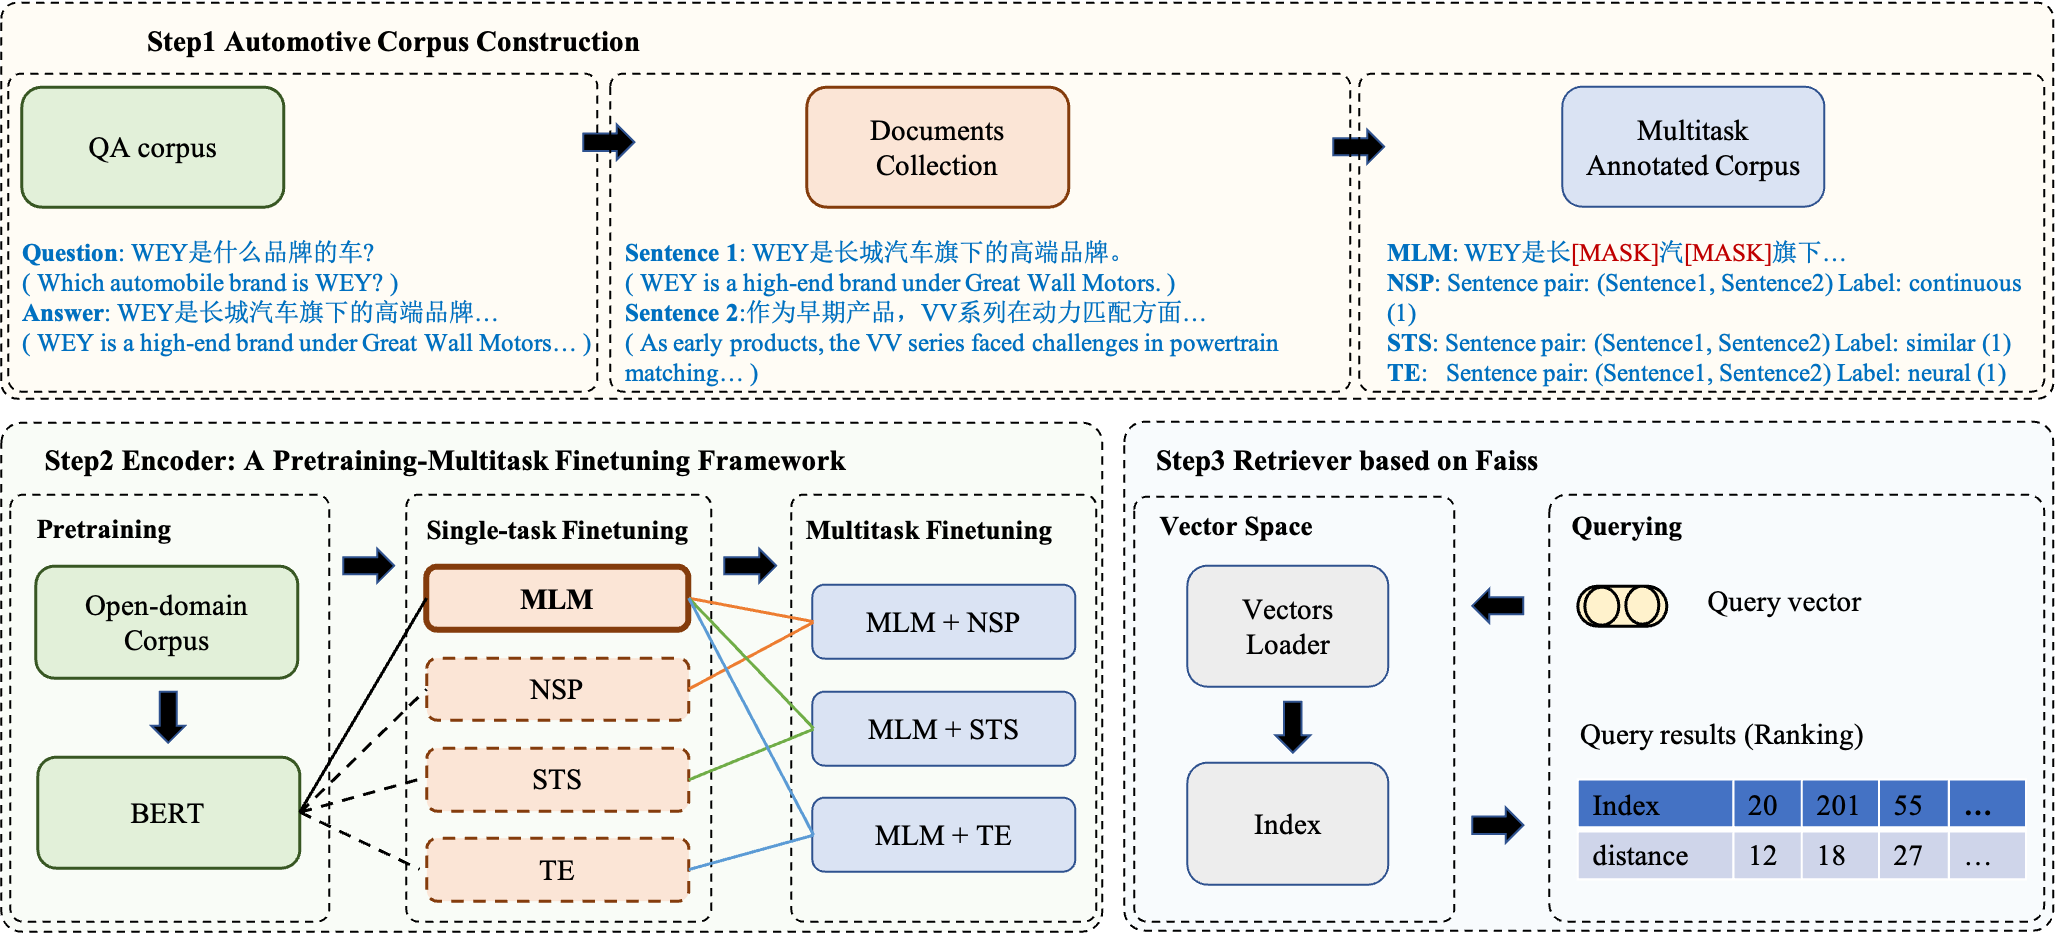
\includegraphics[width=14.0cm]{overview}
	\caption{An overview of our automatic information augmentation framework. \textbf{(a) Step 1}: Interact with ChatGPT to Get Auxiliary Information. \textbf{(b) Step 2}: Distilling the Information and Injecting Them into Context \textbf{(c) Step 3}: Input the Augmented Context into Tagging Model}
	\label{fig:overview}
\end{figure}   


%\unskip
	Existing extractive multi-span question answering models exhibit subpar performance in handling ambiguous words, complex proper nouns (such as film and song titles), numerical values, and long descriptive answers. The main reasons for these shortcomings can be categorized into three aspects:
	\begin{enumerate}
		\item Ambiguous Words: The real world is replete with words that have a single form but multiple meanings, which heavily depend on the context. For instance, the word "Cameron" could refer to a famous director or a former British Prime Minister, depending on the context. The specific meanings of such words often appear infrequently in training corpora, making them difficult to learn.
		\item Numerical Values: In contrast to ambiguous words, numerical values have a single meaning but can be represented in various forms. For example, "22.5 billion years" can also be expressed as "cosmic years".
		\item Multi-span Answers: In extractive multi-span question answering tasks, the model needs to grasp the overall relationship of multi-span answers in the context, such as parallelism and progression.
		These challenges require the model to possess a high level of comprehensive understanding ability and knowledge about language and the world.
	\end{enumerate}
	
	Leveraging large language models to parse question-answering data and inject auxiliary knowledge into the model can promote the integration of the model's latent world knowledge and specific domain knowledge in the paragraph, thereby enhancing the model's performance. Overall, we use GPT-3.5-turbo to generate entity annotations, entity association analysis, and content continuation for each question-answering paragraph as auxiliary information for the model:
	\begin{enumerate}
		\item Context Supplementary: By inserting explanations of entities in the form of annotations after the main entities or concept words in the question and paragraph, this method helps the model capture the actual meaning of ambiguous words in specific contexts. It provides direct information prompts for low-frequency meanings or low-frequency words, achieving entity or concept alignment in the question-answering system.
		\item Context Enrichment: By integrating entity association analysis and content continuation with the original question-answering text to form new paragraphs based on knowledge enhancement, this method captures the inherent associations between words or entity concepts with the same meaning but different forms. On one hand, it parses the logical relationships between other entities using entity relationship analysis. On the other hand, it extends the original paragraph information using content continuation, introducing more external knowledge while helping the model understand the overall content direction of the paragraph, thereby enhancing the model's comprehension ability.
	\end{enumerate}
	

\subsection{Corpus Construction}
\label{sec:corpus_construction}





\section{Experiments}
In this section, we compare our information augmentation approach with multiple strong baseline on multi-span question answering. We first introduce the datasets and experiment setup, then show the experimental results and analysis for different model.

\subsection{Evaluation Dataset}
\label{sec:datasets}
	 We conducted experiments on MultiSpanQA(Li et al., 2022), a recently introduced Reading Comprehension dataset designed for multi-span question answering. This dataset comprises 6.5K multi-span examples in which the questions represent user queries issued to the Google search engine, and the contexts are extracted from the English Wikipedia. It's worth noting that there is a expand variant of MultiSpanQA known as MultispanQA(expand), which intakes single-span and answerable questions. However, we did not perform a comparison with the expanded dataset due to its relatively lower proportion of multi-span QA pairs.

\subsection{Experimental Setup}
	For all competing models and our model, we use the HuggingFace implementation of $\text{BERT}_{base}$ or $\text{RoBERTa}_{base}$ as the \textit{encoder} with $\textit{max\_len}$ = 512. We set the initial learning rate as $3 \times 10^{-5}$ and  $\textit{batch\_size}$ = 4, and use the BERTAdam optimizer with a weight decay of 0.01. Our approach does not involve tuning the parameters on the validation set. Instead, we rely on the model checkpoints obtained after 5 epochs. Next, we introduce the comparison model and evaluation metrics in our experiments.
	
	\subsubsection{\textit{Model Under Comparison}}
	\label{sec:baselines}
	We introduce two comstracting models approaches to multi-span answer extraction : \textbf{TASE} (Segal et al., 2020) and \textbf{LIQUID}(Lee et al., 2023). TASE utilizes a tag-based span extraction model which identifies multi-span answers though the assigning a tag to every input token with BIO tagging scheme. On the other hand, LIQUID serves as a framework for generating multi-span QA datasets to improve model performance.
	
	To enhance the context with auxiliary information, we employ two distinct   approaches: \textbf{$\text{AUG}_{c}$} and \textbf{$\text{AUG}_{eree}$}, where \textbf{AUG} is our automatic data augmentation framework,and the suffix indicates which kind of information is injected into the context. \textbf{$\text{AUG}_{C}$} enriches the context with continue writing, while \textbf{$\text{AUG}_{EREE}$} supplements context with entities information including explanation and relationship analysis.
	Specifically, we leverage ChatGPT as a knowledge source to linearize the relevant information from large language models. in texts format and seamlessly integrate into the original contexts, thus reinforces the information of model inputs.

	
	\subsubsection{\textit{Evaluation Metrics}}
	\label{sec:metrics}
	We use two automatic metrics for evaluation: Exact Match and Overlap F1 score.
	\begin{itemize}
		\item \textbf{Exact Match}. An exact match occurs when a predicted span fully matches one of the ground-truth
		answer spans. We calculate the micro-average precision, recall and f1 score for the extract match
		metric.
		
		\item \textbf{Overlap F1 score}. Overlap F1 score is the macro-average f1 score, where the f1 score for each
		example is computed by treating the prediction and gold as a bag of tokens.
	\end{itemize}

\subsection{Experimental Results and Analysis}
	In this section, we compare $\text{AUG}$ with all competing models described above quantitatively.
	
	\subsubsection{\textit{Comparison Results}}
	We evaluate our model as well as baselines 
	\(( Section ~\ref{sec:baselines} )\) on the development splits of multi-span datasets \(( Section  ~\ref{sec:datasets})\) using automatic metrics \(( Section ~\ref{sec:datasets})\). The comparison results are shown in Table \ref{tab:bertall}, Table \ref{tab:robertaall}.
	
	\begin{table}[H] 
		\caption{Approach performance on complete MultiSpanQA valid set based on $\text{BERT}_{base}$.} 
		\label{tab:bertall}
		\newcolumntype{C}{>{\centering\arraybackslash}X}
		\begin{tabularx}{\textwidth}{p{1.5cm}CCCCCCCC}
			\toprule
			\multirow{2}{*}{\textbf{Model}} & \multicolumn{3}{c}{Exact Match} & \multicolumn{3}{c}{Partial Match}  \\
			\cline{2-7} 
			\addlinespace
			& F\((\%)\)           & P\((\%)\)          & R\((\%)\)           & F\((\%)\)          & P\((\%)\)           & R\((\%)\)           \\
			\midrule
			TASE   & 60.28         & 55.59         & 65.83         & 78.16         & 78.27         & 78.06         \\ 
			LIQUID & 61.44         & 58.39         & 64.84         & 78.56         & 78.65         & 78.46         \\
			$\text{AUG}_{c}$ & 63.05         & 58.51         & 68.34         & 79.42         & 78.70         & 80.14         \\
			$\text{AUG}_{eree}$  & 63.93          & 60.22         & 68.13          & 77.50         & 77.07          & 77.94         \\
			$\text{AUG}_{ereec}$ & 62.90          & 61.02        & 64.89          & 76.72         & 78.56          & 74.97         \\
			Bagging & 64.44          & 61.63        & 67.50          & 79.52         & 80.49          & 78.57         \\
			\bottomrule
		\end{tabularx}
		%	\noindent{\footnotesize{\textsuperscript{1} Tables may have a footer.}}
	\end{table}
	
	\begin{table}[H] 
		\caption{Approach performance on complete MultiSpanQA valid set based on $\text{RoBERTa}_{base}$.} 
		\label{tab:robertaall}
		\newcolumntype{C}{>{\centering\arraybackslash}X}
		\begin{tabularx}{\textwidth}{p{1.5cm}CCCCCCC}
			\toprule
			\multirow{2}{*}{\textbf{Model}} & \multicolumn{3}{c}{Exact Match} & \multicolumn{3}{c}{Partial Match}  \\
			\cline{2-7} 
			\addlinespace
			& F\((\%)\) & P\((\%)\) & R\((\%)\) & F\((\%)\) & P\((\%)\) & R\((\%)\) \\
			\midrule
			TASE & 68.00 & 65.06 & 71.22 & 83.13 & 83.05 & 83.22 \\ 
			LIQUID & 68.33 & 66.68 & 70.07 & 82.71 & 82.45 & 82.98 \\
			$\text{AUG}_{c}$ & 70.35 & 67.35 & 73.63 & 84.06 & 83.38 & 84.76 \\
			$\text{AUG}_{eree}$ & 69.15 & 67.81 & 70.54 & 82.85 & 83.90 & 81.83 \\
			$\text{AUG}_{ereec}$ & 70.44 & 67.83 & 73.26 & 82.80 & 82.45 & 83.15 \\
			Bagging & 70.86 & 69.03 & 72.79 & 84.82 & 85.53 & 84.12 \\
			\bottomrule
		\end{tabularx}      
		%	\noindent{\footnotesize{\textsuperscript{1} Tables may have a footer.}}
	\end{table}
	Table~\ref{tab:bertall} and Table~\ref{tab:robertaall} illustrate the performance comparison between the proposed approaches, $\text{AUG}_{c}$ and $\text{AUG}_{eree}$, and several strong baselines, including the previous state-of-the-art model LIQUID. These comparisons are conducted using both the $\text{BERT}_{base}$ and $\text{RoBERTa}_{base}$ encoders, and regard multi-span question answering as a \textit{BIO} sequence tagging task to predict each token whether it is a part or begin of an answer. 
	Notably,$\text{AUG}_{c}$ exhibit superior performance across the evaluate dataset on all metrics. However, on Partial Match scores, $\text{AUG}_{eree}$ demonstrates slightly lower performance compared to TASE, and especially lower than LIQUID when employing the $\text{BERT}_{base}$ encoder.
	Importantly, the performance of $\text{AUG}_{c}$ consistently outperforms LIQUID and TASE on all metrics and encoders, irrespective of the encoder setting.
	These results demonstrate the effectiveness of our proposed framework, as well as the efficacy of the information augmentation strategy.
	 
	To be more specific, Table~\ref{tab:bertall} shows comparisons of metrics among all competing models 100 backed by $\text{BERT}_{base}$. We can see that our proposed framework, AUG, consistently outperforms all other baselines across multispanQA dataset. Backed by $\text{BERT}_{base}$, $\text{AUG}_{c}$ achieves EM and Overlap F1 scores of 63.05 and 79.42, respectively. Moreover, when equipped with entities’ information,  $\text{AUG}_{eree}$ achieves even higher EM F1 scores of 63.93 but relatively lower Overlap F1 of 77.50 than baselines on the same encoder. These results showcase substantial improvements over the previous state-of-the-art model, LIQUID, with EM F1 score enhancements ranging from 1.61 to 2.49 percents across validation datasets. 
	
	Additionally, when utilizing $\text{RoBERTa}_{base}$ instead of $\text{BERT}_{base}$, $\text{AUG}_{c}$ achieves EM and Overlap F1 scores of 70.35 and 84.06 respectively on the same datasets. These scores represent EM and Overlap F1 improvements of 2.02 and 0.93 compared to the previous setup. For  $\text{AUG}_{eree}$, the EM F1 score represents an enhancement of 0.82, with the EM and Overlap F1 values of 69.16 and 82.85 respectively. Notably, the partial metrics also indicate lower values compared to TASE and LIQUID, in line with the result supported by $\text{BERT}_{base}$. This is because augmenting the model with entity information, including definition and relationship knowledge, strengthens its ability to capture and understand entity concepts, which leads the model to prefer complete entity spans as answers rather than partial entity span, and therefore a decrease in the partial recall and ultimately a lower partial F1 scores and a higher EM F1.
	
	Totally, the result, displayed in Table~\ref{tab:robertaall} demonstrates the same trends to Table~\ref{tab:bertall}. And the outcome highlights robustness in effectively generalizing across different datasets without requiring hyperparameter re-tuning. 
	
\subsubsection{\textit{Discussion}}
	Besides, Table~\ref{tab:bertall} and Table~\ref{tab:robertaall} also discuss the performance of different augmentation integrated strategies, including the results-bagging methods whose outputs are voting results of $\text{AUG}_{c}$, $\text{AUG}_{eree}$ as well as LIQUID, and the input-fusion model $\text{AUG}_{ceree}$ who injects all kinds of information above into input contexts.
	
	In detail, with EM f1 scores of 62.90 and 64.44 in Table~\ref{tab:bertall} and 70.44 and 70.86 in Table~\ref{tab:robertaall}, both the $\text{AUG}_{ceree}$ and Bagging methods consistently surpass TASE and LIQUID, which exhibits robust effectiveness of information injection strategies. However, there is a little decrease caused by fusing all auxiliary information when contrast with single information augmentation strategies and the bagging method. This may be due to the likelihood that incorporating all of the augmentation information into the model inputs will confuse the model by introducing excessive auxiliary knowledge and underrepresented original context proportion. Therefore it may be more useful that adding limit information into context, and using result-bagging method, a multi-model voting to bringing all information into model with an indirect way.
	
	From the Partial Match perspective, $\text{AUG}_{ceree}$ and the Bagging method achieve 76.72 and 79.52 in Table~\ref{tab:bertall}, and 82.80 and 84.82 in Table~\ref{tab:robertaall}. In accordance with Exact Match metrics, Bagging demonstrate a overall superior performance. Meanwhile overlap f1 score of $\text{AUG}_{eree}$ is inferior to TASE but superior to LIQUID ,with relatively higher precision and relativelv higher recall, which  is comparable to all single augmented models such as $\text{AUG}_{eree}$. And its weak performance on overlap f1 also reveals complete entities preference of this information injection approach.
	z
	In addition, we	categorized the data in MultispanQA into DESC, NUM, ENTYS in terms of answer types, and compared the performance of each of the model mentioned above in each breakdown category. Specifically,  Table~\ref{tab:bertsub} and Table~\ref{tab:robertasub} present the results backed by  $\text{BERT}_{base}$ and $\text{RoBERTa}_{base}$, respectively. As shown in Tables~\ref{tab:bertsub},Table~\ref{tab:robertasub}, our proposed models display superior performance in DESC and ENTYS categories answer extraction, which to some extent indicates the enhancement of models' knowledge at entity and description levels.
	
	\textcolor{red}{please supplements new overlap calculation method in tase-zh}
	
	\begin{table}[ht]
		\caption{Model performance on complete MultiSpanQA valid Subset with different answer types based on $\text{BERT}_{base}$.}
		\label{tab:bertsub}
		\newcolumntype{C}{>{\centering\arraybackslash}X}
		\begin{tabularx}{\textwidth}{Cp{1.5cm}CCCCCCC}
			\toprule
			\multirow{2}{*}{\textbf{Type}} & \multirow{2}{*}{\textbf{Model}} & \multicolumn{3}{c}{Exact Match} & \multicolumn{3}{c}{Partial Match} \\
			\cmidrule{3-8} 
			& & F\((\%)\) & P\((\%)\) & R\((\%)\) & F\((\%)\) & P\((\%)\) & R\((\%)\) \\
			\midrule
			\multirow{6}{*}{DESC} & TASE & 32.76 & 27.33 & 40.87 & 64.46 & 68.61 & 60.79 \\ 
			& LIQUID & 36.69 & 31.10 & 44.71 & 66.05 & 65.95 & 66.15 \\
			& $\text{AUG}_{c}$ & 38.74 & 32.89 & 47.12 & 68.31 & 70.32 & 66.42 \\
			& $\text{AUG}_{eree}$ & 44.69 & 40.71 & 49.52 & 63.12 & 67.16 & 59.53 \\
			& $\text{AUG}_{ereec}$ & 40.63 & 38.30 & 43.27 & 64.25 & 71.15 & 58.57 \\
			& Bagging & 39.91 & 36.69 & 43.75 & 66.70 & 73.68 & 60.93 \\
			\midrule
			\multirow{6}{*}{NUM} & TASE & 33.33 & 30.23 & 37.14 & 60.98 & 71.99 & 52.89 \\ 
			& LIQUID & 34.33 & 31.25 & 38.10 & 60.68 & 68.15 & 54.69 \\
			& $\text{AUG}_{c}$ & 35.96 & 33.33 & 39.05 & 64.47 & 71.56 & 58.65 \\
			& $\text{AUG}_{eree}$ & 36.20 & 34.48 & 38.10 & 59.02 & 65.63 & 53.62 \\
			& $\text{AUG}_{ereec}$ & 36.71 & 37.25 & 36.19 & 57.09 & 69.04 & 48.67 \\
			& Bagging & 35.94 & 34.82 & 37.14 & 60.73 & 71.15 & 52.97 \\
			\midrule
			\multirow{6}{*}{ENTYS} & TASE & 66.30 & 62.21 & 70.96 & 81.16 & 80.37 & 81.96 \\ 
			& LIQUID & 67.17 & 65.25 & 69.21 & 81.66 & 81.69 & 81.63 \\
			& $\text{AUG}_{c}$ & 68.47 & 64.44 & 73.03 & 81.93 & 80.57 & 83.34 \\
			& $\text{AUG}_{eree}$ & 68.36 & 64.64 & 72.53 & 80.55 & 79.21 & 81.93 \\
			& $\text{AUG}_{ereec}$ & 67.54 & 65.60 & 69.59 & 79.49 & 80.16 & 78.83 \\
			& Bagging & 69.65 & 66.94 & 72.59 & 82.31 & 82.07 & 82.55 \\
			\bottomrule
		\end{tabularx}
	\end{table}
	
	\begin{table}[ht]
		\caption{Model performance on complete MultiSpanQA valid Subset with different answer types based on $\text{RoBERTa}_{base}$.}
		\label{tab:robertasub}
		\newcolumntype{C}{>{\centering\arraybackslash}X}
		\begin{tabularx}{\textwidth}{Cp{1.5cm}CCCCCCC}
			\toprule
			\multirow{2}{*}{\textbf{Type}} & \multirow{2}{*}{\textbf{Model}} & \multicolumn{3}{c}{Exact Match} & \multicolumn{3}{c}{Partial Match} \\
			\cmidrule{3-8} 
			& & F\((\%)\) & P\((\%)\) & R\((\%)\) & F\((\%)\) & P\((\%)\) & R\((\%)\) \\
			\midrule
			\multirow{6}{*}{DESC} & TASE & 45.53 & 40.84 & 51.44 & 75.44 & 76.61 & 74.31 \\ 
			& LIQUID & 48.68 & 44.76 & 53.37 & 73.27 & 71.57 & 75.04 \\
			& $\text{AUG}_{c}$ & 49.02 & 44.66 & 54.33 & 76.33 & 77.85 & 74.86 \\
			& $\text{AUG}_{eree}$ & 50.99 & 46.96 & 55.77 & 76.87 & 78.07 & 75.71 \\
			& $\text{AUG}_{ereec}$ & 49.24 & 44.71 & 54.81 & 71.87 & 73.03 & 70.74 \\
			& Bagging & 47.70 & 43.78 & 52.40 & 77.43 & 80.63 & 74.47 \\
			\midrule
			\multirow{6}{*}{NUM} & TASE & 46.23 & 45.79 & 46.67 & 71.89 & 78.42 & 66.36 \\ 
			& LIQUID & 40.19 & 39.45 & 40.95 & 67.56 & 72.28 & 63.42 \\
			& $\text{AUG}_{c}$ & 50.69 & 49.11 & 52.38 & 72.86 & 80.22 & 66.74 \\
			& $\text{AUG}_{eree}$ & 42.40 & 41.07 & 43.81 & 66.67 & 73.51 & 61.00 \\
			& $\text{AUG}_{ereec}$ & 45.58 & 44.55 & 46.67 & 65.86 & 73.19 & 59.87 \\
			& Bagging & 44.65 & 43.64 & 45.71 & 70.11 & 78.49 & 63.35 \\
			\midrule
			\multirow{6}{*}{ENTYS} & TASE & 72.57 & 69.94 & 75.41 & 84.90 & 84.32 & 85.48 \\ 
			& LIQUID & 72.95 & 71.77 & 74.16 & 85.02 & 84.75 & 85.29 \\
			& $\text{AUG}_{c}$ & 74.59 & 71.87 & 77.53 & 85.79 & 84.40 & 87.23 \\
			& $\text{AUG}_{eree}$ & 73.50 & 72.81 & 74.22 & 84.74 & 85.49 & 83.99 \\
			& $\text{AUG}_{ereec}$ & 75.04 & 72.81 & 77.41 & 85.37 & 84.46 & 86.29 \\
			& Bagging & 75.85 & 74.52 & 77.22 & 86.73 & 86.73 & 86.74 \\
			\bottomrule
		\end{tabularx}
	\end{table}

\subsubsection{\textit{Ablation Experiment}}
	At the end of this section, we conducted ablations on our approach to confirm the effectiveness of selecting the information injection proportion. For each QA data, we randomly split the original context and the auxiliary text, then concatenated them into a final augmented context with a specific proportion to ensure that the new input length meets $\textit{max\_len}$, which has a crucial impact on our approach. In practice, we determined the final text splicing ratio by calculating the ratio of the average length of the source text to the added information, which for the $\text{AUG}_{c}$ is 0.86.
	
	Specifically, Table~\ref{tab:different_ratio_bert} and Table~\ref{tab:different_ratio_roberta} displays $\text{AUG}_{c}$'s performance with differential proportion to concatenate original contexts and continuation, on complete MultispanQA valid set,backed by $\text{BERT}_{base}$ and $\text{RoBERTa}_{base}$ respectively. We choose five proportions for information integration, which determine how much auxiliary information would be inject into each overflowed text segment. The results presented in tables indicate that using the ratio of their average lengths as the proportion of the overflow text composed of original text and auxiliary information is an effective approach. In detail, $\text{AUG}_{c}$,equipping with $\text{BERT}_{base}$, achieves an Exact Match F1 scores improvements of at least 4.57 compared to other proportions and an overlap F1 scores improvements of at least 2.07. In line with Table~\ref{tab:different_ratio_bert}, when $\text{AUG}_{c}$ equips with $\text{Roberta}_{base}$, it achieves an improvement of Exact Match F1 scores of 0.55 but an decrease of Overlap F1 scores of 0.17.

	

\begin{table}[H] 
	\caption{Ablations of $\text{AUG}_{c}$ on different proportion for information concatenation, based on $\text{BERT}_{base}$.} 
	\label{tab:different_ratio_bert}
	\newcolumntype{C}{>{\centering\arraybackslash}X}
	\begin{tabularx}{\textwidth}{p{1.7cm}CCCCCCC}
		\toprule
		\multirow{2}{*}{\textbf{Proportion}} & \multicolumn{3}{c}{Exact Match} & \multicolumn{3}{c}{Partial Match}  \\
		\cline{2-7} 
		\addlinespace
		& F\((\%)\) & P\((\%)\) & R\((\%)\) & F\((\%)\) & P\((\%)\) & R\((\%)\) \\
		\midrule
		0.90 & 58.55 & 57.69 & 59.44 & 71.88 & 74.30 & 69.61 \\ 
		0.70 & 61.70 & 59.03 & 64.63 & 76.58 & 77.84 & 75.36 \\
		0.50 & 61.22 & 57.37 & 65.62 & 77.38 & 77.61 & 77.16 \\
		0.40 & 61.36 & 56.50 & 67.13 & 78.26 & 77.57 & 78.96 \\
		0.10 & 61.41 & 56.36 & 67.45 & 78.94 & 78.45 & 79.44 \\
		0.14 & 63.05 & 58.51 & 68.34 & 79.42 & 78.70 & 80.14 \\
		\bottomrule
	\end{tabularx}      
	%	\noindent{\footnotesize{\textsuperscript{1} Tables may have a footer.}}
\end{table}



\begin{table}[H] 
	\caption{Ablations of $\text{AUG}_{c}$ on different proportion for information concatenation, based on $\text{BERT}_{base}$.} 
	\label{tab:different_ratio_roberta}
	\newcolumntype{C}{>{\centering\arraybackslash}X}
	\begin{tabularx}{\textwidth}{p{1.7cm}CCCCCCC}
		\toprule
		\multirow{2}{*}{\textbf{Proportion}} & \multicolumn{3}{c}{Exact Match} & \multicolumn{3}{c}{Partial Match}  \\
		\cline{2-7} 
		\addlinespace
		& F\((\%)\) & P\((\%)\) & R\((\%)\) & F\((\%)\) & P\((\%)\) & R\((\%)\) \\
		\midrule
		0.90 & 58.13 & 56.92 & 59.39 & 71.70 & 73.49 & 69.98 \\ 
		0.70 & 66.97 & 65.42 & 68.60 & 80.05 & 80.80 & 79.32 \\
		0.50 & 68.94 & 67.23 & 70.75 & 82.43 & 83.23 & 81.64 \\
		0.40 & 68.95 & 66.11 & 71.06 & 83.71 & 83.71 & 81.71 \\
		0.10 & 69.80 & 66.47 & 73.47 & 84.23 & 83.49 & 84.99 \\
		0.86 & 70.35 & 67.35 & 73.63 & 84.06 & 83.38 & 84.76 \\
		\bottomrule
	\end{tabularx}      
	%	\noindent{\footnotesize{\textsuperscript{1} Tables may have a footer.}}
\end{table}

\section{Conclusion}


%All figures and tables should be cited in the main text as Figure~\ref{fig1}, Table~\ref{tab1}, etc.

%\section{Discussion}
%
%Authors should discuss the results and how they can be interpreted from the perspective of previous studies and of the working hypotheses. The findings and their implications should be discussed in the broadest context possible. Future research directions may also be highlighted.

%%%%%%%%%%%%%%%%%%%%%%%%%%%%%%%%%%%%%%%%%%
%\section{Conclusions}
%
%This section is not mandatory, but can be added to the manuscript if the discussion is unusually long or complex.


%%%%%%%%%%%%%%%%%%%%%%%%%%%%%%%%%%%%%%%%%%
\vspace{6pt} 

%%%%%%%%%%%%%%%%%%%%%%%%%%%%%%%%%%%%%%%%%%
%% optional
%\supplementary{The following supporting information can be downloaded at:  \linksupplementary{s1}, Figure S1: title; Table S1: title; Video S1: title.}

% Only for journal Methods and Protocols:
% If you wish to submit a video article, please do so with any other supplementary material.
% \supplementary{The following supporting information can be downloaded at: \linksupplementary{s1}, Figure S1: title; Table S1: title; Video S1: title. A supporting video article is available at doi: link.}

% Only for journal Hardware:
% If you wish to submit a video article, please do so with any other supplementary material.
% \supplementary{The following supporting information can be downloaded at: \linksupplementary{s1}, Figure S1: title; Table S1: title; Video S1: title.\vspace{6pt}\\
%\begin{tabularx}{\textwidth}{lll}
%\toprule
%\textbf{Name} & \textbf{Type} & \textbf{Description} \\
%\midrule
%S1 & Python script (.py) & Script of python source code used in XX \\
%S2 & Text (.txt) & Script of modelling code used to make Figure X \\
%S3 & Text (.txt) & Raw data from experiment X \\
%S4 & Video (.mp4) & Video demonstrating the hardware in use \\
%... & ... & ... \\
%\bottomrule
%\end{tabularx}
%}

%%%%%%%%%%%%%%%%%%%%%%%%%%%%%%%%%%%%%%%%%%
%\authorcontributions{For research articles with several authors, a short paragraph specifying their individual contributions must be provided. The following statements should be used ``Conceptualization, X.X. and Y.Y.; methodology, X.X.; software, X.X.; validation, X.X., Y.Y. and Z.Z.; formal analysis, X.X.; investigation, X.X.; resources, X.X.; data curation, X.X.; writing---original draft preparation, X.X.; writing---review and editing, X.X.; visualization, X.X.; supervision, X.X.; project administration, X.X.; funding acquisition, Y.Y. All authors have read and agreed to the published version of the manuscript.'', please turn to the  \href{http://img.mdpi.org/data/contributor-role-instruction.pdf}{CRediT taxonomy} for the term explanation. Authorship must be limited to those who have contributed substantially to the work~reported.}

\funding{ This research was supported by the Natural Science Foundation of Zhejiang Province, China (Grant No. LQ22F020027) and the Key Research and Development Program of Zhejiang Province, China (2023C01041).}


%\acknowledgments{In this section you can acknowledge any support given which is not covered by the author contribution or funding sections. This may include administrative and technical support, or donations in kind (e.g., materials used for experiments).}

\conflictsofinterest{The authors declare no conflict of interest.} 

%%%%%%%%%%%%%%%%%%%%%%%%%%%%%%%%%%%%%%%%%%


%% Only for journal Encyclopedia
%\entrylink{The Link to this entry published on the encyclopedia platform.}



%%%%%%%%%%%%%%%%%%%%%%%%%%%%%%%%%%%%%%%%%%
\begin{adjustwidth}{-\extralength}{0cm}
%\printendnotes[custom] % Un-comment to print a list of endnotes

\reftitle{References}

% Please provide either the correct journal abbreviation (e.g. according to the “List of Title Word Abbreviations” http://www.issn.org/services/online-services/access-to-the-ltwa/) or the full name of the journal.
% Citations and References in Supplementary files are permitted provided that they also appear in the reference list here. 

%=====================================
% References, variant A: external bibliography
%=====================================
%\bibliography{your_external_BibTeX_file}

%=====================================
% References, variant B: internal bibliography
%=====================================
\begin{thebibliography}{999}
	% Reference 1
	\bibitem[Gupta(2005)]{asq-system}
	Gupta, N.; Tur, G.; Hakkani-Tur, D.; et al. The AT\&T spoken language understanding system. {\em IEEE Transactions on Audio, Speech, and Language Processing}, {\bf 2005}, {\em 14(1)}, 213-222.
	\bibitem[Ferrucci(2010)]{watson}
	Ferrucci, D.G.; Brown, E.; Chu-Carroll, J.; Fan, J.; Gondek, D.; Kalyanpur, A.A.; Lally, A.; Murdock, J.W.; Nyberg, E.; Prager, J.; Schlaefer, N.; Welty, C. Building Watson: An Overview of the DeepQA Project. {\em AI Magazine} {\bf 2010}, {\em 31(3)}, 59--79.
	\bibitem[Qu(2018)]{odqa2018}
	Qu, C.; Yang, L.; Qiu, M.H. Open domain question answering using early fusion of knowledge bases and text. Available online: https://doi.org/10.48550/arXiv.1809.00782. (accessed on 19-05-2023).
	\bibitem[Vaswani(2017)]{transformers2017}
	Vaswani, A.; Shazeer, N.; Parmar, N.; Uszkoreit, J.; Jones, L.; Gomez, A.N.; Polosukhin, I. Attention Is All You Need. In Proceedings of Advances in Neural Information Processing Systems(ANIPS), California, USA, 2017; 5998-6008.
	\bibitem[Devlin(2019)]{bert2019}
	Devlin, J.; Chang, M.W.; Lee, K.; Toutanova, K. BERT: Pre-training of Deep Bidirectional Transformers for Language Understanding. In Proceedings of the Conference of the North American Chapter of the Association for Computational Linguistics: Human Language Technologies (NAACL-HLT), Minneapolis, 2019; 4171-4186.
	\bibitem[Radford(2018)]{gpt}
	Radford, A.; Narasimhan, K.; Salimans, T.; Sutskever, I. Improving Language Understanding by Generative Pre-Training. Available online: https://cdn.openai.com/research-covers/language-unsupervised/language\_understanding\_paper.pdf. (accessed on 19-05-2023).
	\bibitem[Radford(2020)]{gpt2}
	Radford, A.; Wu, J.; Child, R.; Luan, D.; Amodei, D.; Sutskever, I. Language Models are Unsupervised Multitask Learners. Available online: https://cdn.openai.com/better-language-models/language\_models\_are\_unsupervised\_multitask\_learners.\\pdf. (accessed on 19-05-2023).
	\bibitem[Brown(2020)]{gpt3}
	Brown, T.; Mann, B.; Ryder, N.; et al. Language models are few-shot learners. In proceedings of Advances in Neural Information Processing Systems, Virtual-only Conference, 2020, 33: 1877-1901.
	\bibitem[Rajpurkar(2016)]{squad}
	Rajpurkar, P.; Zhang, J.; Lopyrev, K.; Liang, P. Squad: 100,000+ questions for machine comprehension of text. In Proceedings of the Conference on Empirical Methods in Natural Language Processing(EMNLP), Austin, Texas, USA, 2016, 2383-2392.
	\bibitem[Rajpurkar(2018)]{squad2.0}
	Rajpurkar, P.; Jia, R.; Liang, P. Know what you don’t know: Unanswerable questions for squad. In Proceedings of the 56th Annual Meeting of the Association for Computational Linguistics (Volume 2: Short Papers), Melbourne, Australia, 2018, 784–789.
	\bibitem[Li(2022)]{multispanqa}
	Li, H.; Tomko, M.; Vasardani, M.; Baldwin, T. MultiSpanQA: A dataset for multi-span question answering. In Proceedings of the Conference of the North American Chapter of the Association for Computational Linguistics: Human Language Technologies (NAACL-HLT), Seattle, Washington, 2022, 1250–1260.
	\bibitem[Yang(2019)]{bertserini}
	Yang, Wei; et al. End-to-end open-domain question answering with bertserini. Available online: https://doi.org/10.48550/ar-\\Xiv.1902.01718. (accessed on 19-05-2023).
	\bibitem[Zhang(2022)]{qa-survey}
	Zhang, Q.; Chen, S.S.; Xu, D.K.; Cao, Q.Q.; Chen, X.J.; Cohn, T.; Fang, M. A Survey for Efficient Open Domain Question Answering. Available Online: https://arxiv.org/abs/2211.07886. (accessed on 19-05-2023).
	\bibitem[Jones(1972)]{tf-idf}
	Jones, S.K. A statistical interpretation of term specificity and its application in retrieval. {\em Journal of Documentation} {\bf 1972}, {\em 28(1)}, 11--21.
%	\bibitem[Lin(2017)]{multichannel}
%	Lin, B. Y.; Xu, F. F.; Luo, Z.; et al. Multi-channel bilstm-crf model for emerging named entity recognition in social media. In Proceedings of the 3rd Workshop on Noisy User-generated Text, Copenhagen, Denmark, 2017, 160-165.
	\bibitem[Baldwin(2015)]{hand-crafted-features}
	Baldwin, T.; Marneffe M.C.; Han, B.; et al. Shared tasks of the 2015 workshop on noisy user-generated text: Twitter lexical normalization and named entity recognition. In Proceedings of the workshop on noisy user-generated text, Beijing, China, 2015, 126-135.
	\bibitem[Derczynski(2015)]{tweet}
	Derczynski, L.; Maynard, D.; Rizzo, G.; et al. Analysis of named entity recognition and linking for tweets. {\em Information Processing \& Management} {\bf 2015}, {\em 51(2)}, 32-49.
	\bibitem[Mikolov(2013)]{word2vec}
	Mikolov, T.; Chen, K.; Corrado, G.; Dean, J. Efficient estimation of word representations in vector space. Available online: https://arxiv.org/abs/1301.3781. (accessed on 19-05-2023).
%	\bibitem[Le(2014)]{word2vec2}
%	Le, Q.; Mikolov, T. Distributed representations of sentences and documents. In Proceedings of the 31st International Conference on Machine Learning (ICML), Beijing, China, 2014; 1188-1196.
	\bibitem[Harris(1954)]{distributed-hypothesis}
	Harris, Z.S. Distributional structure. {\em Journal of Documentation} {\bf 1954}, {\em 10(2-3)}, 146--162.
	\bibitem[Le(2014)]{glove}
	Pennington, J.; Socher, R.; Manning, C.D. GloVe: Global Vectors for Word Representation. In Proceedings of the 2014 conference on empirical methods in natural language processing (EMNLP),  Maryland, USA, 2014; 1532-1543.
	\bibitem[Vaswani(2017)]{cove}
	McCann, B.; Bradbury, J.; Xiong, C.; Socher, R. Learned in translation: Contextualized word vectors. In Proceedings of Advances in Neural Information Processing Systems(NIPS), California, USA, 2017; 6297-6308.
	\bibitem[Peters(2018)]{elmo}
	Peters, M.E.; Neumann, M.; Iyyer, M.; Gardner, M.; Clark, C.; Lee, K.; Zettlemoyer, L. Deep contextualized word representations. In Proceedings of the 2018 Conference of the North American Chapter of the Association for Computational Linguistics: Human Language Technologies, New Orleans, USA, 2018; 2227-2237.
	\bibitem[Devika(2021)]{app1}
	Devika, R.; Vairavasundaram, S.; Mahenthar, C.S.J.; et al. A Deep Learning Model Based on BERT and Sentence Transformer for Semantic Keyphrase Extraction on Big Social Data. In  IEEE Access \textbf{2021}, 9, 165252-165261.
	\bibitem[Natarajan(2022)]{app2}
	Natarajan, B.; Rajalakshmi, E.; Elakkiya, R; et al. Development of an End-to-End Deep Learning Framework for Sign Language Recognition, Translation, and Video Generation. In IEEE Access \textbf{2022}, 10, 104358-104374.
	\bibitem[Bentley(1975)]{kd-tree}
	Bentley, J.L. Multidimensional binary search trees used for associative searching. {\em Communications of the ACM} {\bf 1975}, {\em 18(9)}, 509-517.
	\bibitem[Liu(2006)]{ball-tree}
	Liu, T.; Moore, A.W.; Gray, A.; New algorithms for efficient high-dimensional nonparametric classification. {\em JMLR} {\bf 2006}, 7, 1135–1158.
	\bibitem[Omohundro(1989)]{ball-tree2}
	Omohundro SM. Five balltree construction algorithms. Berkeley, California, USA: International Computer Science Institute, 1989.
	\bibitem[Friedman(1977)]{knn-graph}
	Friedman, J.H.; Bentley, J.L.; Finkel, R.A. An algorithm for finding best matches in logarithmic expected time. {\em ACM Transactions on Mathematical Software} {\bf 1977}, {\em 3(3)}, 209-226.
	\bibitem[Jégou(2011)]{pq}
	Jégou, H.; Douze, M.; Schmid, C. Product quantization for nearest neighbor search. {\em IEEE Transactions on Pattern Analysis and Machine Intelligence} {\bf 2011}, {\em 33(1)}, 117-128.
	\bibitem[20Indyk(1998)]{lsh}
	Indyk, P.; Motwani, R. Approximate nearest neighbors: towards removing the curse of dimensionality. In Proceedings of the Thirtieth Annual ACM Symposium on Theory of Computing, New York, USA, 1998; 604-613.
	\bibitem[21Malkov(2018)]{hnsw}
	Malkov, Y.A.; Yashunin, D.A. Efficient and robust approximate nearest neighbor search using Hierarchical Navigable Small World graphs. Available online: https://arxiv.org/abs/1603.09320. (accessed on 19-05-2023).
	\bibitem[Jégou(2010)]{pns}
	Jégou, H.; Perronnin, F.; Douze, M.; Sánchez, J.; Pérez, P.; Schmid, C. Aggregating local descriptors into a compact image representation. In Proceedings of the 2010 IEEE Computer Society Conference on Computer Vision and Pattern Recognition, San Francisco, USA, 2010; 3304-3311.
	\bibitem[Wang(2019)]{haq}
	Wang, K.; Liu, Z.; Lin, Y.; Lin, W.; Han, S. HAQ: Hardware-Aware Automated Quantization with Mixed Precision. In Proceedings of  the IEEE Computer Society Conference on Computer Vision and Pattern Recognition, Los Angeles, USA, 2019; 1669-1678.	
	\bibitem[Johnson(2011)]{faiss}
	Johnson, J.; Douze, M.; Jégou, H. Billion-scale similarity search with GPUs. {\em IEEE Transactions on Big Data} {\bf 2019}, {\em 7(3)}, 535-547.	
%	\bibitem[Zhu(2015)]{}
%	Zhu, Y.K.; Kiros, R.; Zemel, R.; Salakhutdinov, R.; Urtasun, R.; Torralba, A.; Fidler, S. Aligning books and movies: Towards story-like visual explanations by watching movies and reading books. In Proceedings of the IEEE International Conference on Computer Vision, Santiago, Republic of Chile, 2015; 19-27.
	\bibitem[Liu(2019)]{roberta}
	Liu, Y.; Ott, M.; Goyal, N.; Du, J.; Joshi, M.; Chen, D. RoBERTa: A Robustly Optimized BERT Pretraining Approach. Available online: https://arxiv.org/abs/1603.09320. (accessed on 19-05-2023).
	\bibitem[Johnson(2020)]{spanbert}
	Clark, C.; Lee, K.; Chang, M.W.; Kwiatkowski, T.; Collins, M.; Toutanova, K. SpanBERT: Improving Pre-training by Representing and Predicting Spans. {\em Transactions of the Association for Computational Linguistics} {\bf 2020}, {\em 8}, 64-77.
	%	% Reference 2
%	\bibitem[Author2(year)]{ref-book1}
%	Author~2, L. The title of the cited contribution. In {\em The Book Title}; Editor 1, F., Editor 2, A., Eds.; Publishing House: City, Country, 2007; pp. 32--58.
%	% Reference 3
%	\bibitem[Author3(year)]{ref-book2}
%	Author 1, A.; Author 2, B. \textit{Book Title}, 3rd ed.; Publisher: Publisher Location, Country, 2008; pp. 154--196.
%	% Reference 4
%	\bibitem[Author4(year)]{ref-unpublish}
%	Author 1, A.B.; Author 2, C. Title of Unpublished Work. \textit{Abbreviated Journal Name} year, \textit{phrase indicating stage of publication (submitted; accepted; in press)}.
%	% Reference 5
%	\bibitem[Author5(year)]{ref-communication}
%	Author 1, A.B. (University, City, State, Country); Author 2, C. (Institute, City, State, Country). Personal communication, 2012.
%	% Reference 6
%	\bibitem[Author6(year)]{ref-proceeding}
%	Author 1, A.B.; Author 2, C.D.; Author 3, E.F. Title of presentation. In Proceedings of the Name of the Conference, Location of Conference, Country, Date of Conference (Day Month Year); Abstract Number (optional), Pagination (optional).
%	% Reference 7
%	\bibitem[Author7(year)]{ref-thesis}
%	Author 1, A.B. Title of Thesis. Level of Thesis, Degree-Granting University, Location of University, Date of Completion.
%	% Reference 8
%	\bibitem[Author8(year)]{ref-url}
%	Title of Site. Available online: URL (accessed on Day Month Year).
\end{thebibliography}
% Reference 2
%\bibitem[Author2(year)]{ref-book1}
%Author~2, L. The title of the cited contribution. In {\em The Book Title}; Editor 1, F., Editor 2, A., Eds.; Publishing House: City, Country, 2007; pp. 32--58.
%% Reference 3
%\bibitem[Author3(year)]{ref-book2}
%Author 1, A.; Author 2, B. \textit{Book Title}, 3rd ed.; Publisher: Publisher Location, Country, 2008; pp. 154--196.
%% Reference 4
%\bibitem[Author4(year)]{ref-unpublish}
%Author 1, A.B.; Author 2, C. Title of Unpublished Work. \textit{Abbreviated Journal Name} year, \textit{phrase indicating stage of publication (submitted; accepted; in press)}.
%% Reference 5
%\bibitem[Author5(year)]{ref-communication}
%Author 1, A.B. (University, City, State, Country); Author 2, C. (Institute, City, State, Country). Personal communication, 2012.
%% Reference 6
%\bibitem[Author6(year)]{ref-proceeding}
%Author 1, A.B.; Author 2, C.D.; Author 3, E.F. Title of presentation. In Proceedings of the Name of the Conference, Location of Conference, Country, Date of Conference (Day Month Year); Abstract Number (optional), Pagination (optional).
%% Reference 7
%\bibitem[Author7(year)]{ref-thesis}
%Author 1, A.B. Title of Thesis. Level of Thesis, Degree-Granting University, Location of University, Date of Completion.
%% Reference 8
%\bibitem[Author8(year)]{ref-url}
%Title of Site. Available online: URL (accessed on Day Month Year).

% If authors have biography, please use the format below
%\section*{Short Biography of Authors}
%\bio
%{\raisebox{-0.35cm}{\includegraphics[width=3.5cm,height=5.3cm,clip,keepaspectratio]{Definitions/author1.pdf}}}
%{\textbf{Firstname Lastname} Biography of first author}
%
%\bio
%{\raisebox{-0.35cm}{\includegraphics[width=3.5cm,height=5.3cm,clip,keepaspectratio]{Definitions/author2.jpg}}}
%{\textbf{Firstname Lastname} Biography of second author}

% For the MDPI journals use author-date citation, please follow the formatting guidelines on http://www.mdpi.com/authors/references
% To cite two works by the same author: \citeauthor{ref-journal-1a} (\citeyear{ref-journal-1a}, \citeyear{ref-journal-1b}). This produces: Whittaker (1967, 1975)
% To cite two works by the same author with specific pages: \citeauthor{ref-journal-3a} (\citeyear{ref-journal-3a}, p. 328; \citeyear{ref-journal-3b}, p.475). This produces: Wong (1999, p. 328; 2000, p. 475)




%%%%%%%%%%%%%%%%%%%%%%%%%%%%%%%%%%%%%%%%%%
%% for journal Sci
%\reviewreports{\\
%Reviewer 1 comments and authors’ response\\
%Reviewer 2 comments and authors’ response\\
%Reviewer 3 comments and authors’ response
%}
%%%%%%%%%%%%%%%%%%%%%%%%%%%%%%%%%%%%%%%%%%
\PublishersNote{}

\end{adjustwidth}
\end{document}

